% --------------------------------------------------------------
% This is all preamble stuff that you don't have to worry about.
% Head down to where it says "Start here"
% --------------------------------------------------------------
 
\documentclass[12pt]{article}
 \listfiles
\usepackage[margin=1in]{geometry} 
\usepackage{amsmath,amsthm,amssymb,mathtools}
\usepackage{float}
\usepackage{graphicx}
\usepackage{cancel}
\usepackage{tikz}
\usepackage{xcolor}
\usepackage{bm}
\usepackage{tikz}
\usepackage{bm}
\usepackage{cancel}
\usepackage{filecontents}
\usepackage{algorithm}
\usepackage{algpseudocode} % loads algorithmicx

\usepackage{pgfplots}
%\pgfplotsset{compat=1.10}
\usetikzlibrary{intersections}
%\usepgfplotslibrary{fillbetween}

\newcommand{\N}{\mathbb{N}}
\newcommand{\Z}{\mathbb{Z}}
\newcommand{\sign}[1]{\text{sign}(#1)}
\newcommand{\abs}[1]{\left| #1 \right|}
\newcommand{\BigO}[1]{\mathcal{O}\left( #1 \right)}
\renewcommand{\Pr}[1]{\text{Pr}[ #1 ]}
\newcommand{\norm}[1]{\left|\left| #1 \right|\right|}
\newcommand{\inner}[2]{\left< #1 , #2\right>}
\newcommand{\R}{\mathbb{R}}
\newcommand{\grad}{\nabla}
\renewcommand{\P}[1]{\left( #1 \right)}
\newcommand{\B}[1]{\left[ #1 \right]}
 
\newenvironment{theorem}[2][Theorem]{\begin{trivlist}
\item[\hskip \labelsep {\bfseries #1}\hskip \labelsep {\bfseries #2.}]}{\end{trivlist}}
\newenvironment{lemma}[2][Lemma]{\begin{trivlist}
\item[\hskip \labelsep {\bfseries #1}\hskip \labelsep {\bfseries #2.}]}{\end{trivlist}}
\newenvironment{exercise}[2][Exercise]{\begin{trivlist}
\item[\hskip \labelsep {\bfseries #1}\hskip \labelsep {\bfseries #2.}]}{\end{trivlist}}
\newenvironment{problem}[2][Problem]{\begin{trivlist}
\item[\hskip \labelsep {\bfseries #1}\hskip \labelsep {\bfseries #2.}]}{\end{trivlist}}
\newenvironment{question}[2][Question]{\begin{trivlist}
\item[\hskip \labelsep {\bfseries #1}\hskip \labelsep {\bfseries #2.}]}{\end{trivlist}}
\newenvironment{corollary}[2][Corollary]{\begin{trivlist}
\item[\hskip \labelsep {\bfseries #1}\hskip \labelsep {\bfseries #2.}]}{\end{trivlist}}

%\algrenewcommand{\algorithmiccomment}[1]{\hskip3em$\vartriangleright$ #1}
\algnewcommand\algorithmicinput{\textbf{Input:}}
\algnewcommand\Input{\item[\algorithmicinput]}
\algnewcommand\algorithmicoutput{\textbf{Output:}}
\algnewcommand\Output{\item[\algorithmicoutput]}


\begin{filecontents*}{2.1y.dat}
X Y
0 1
1 -0.8
2 1.0
3 -0.8
4 1.0
5 -0.8
6 1.0
7 -0.8
8 1.0
9 -0.8
10 1.0
11 -0.8
12 1.0
13 -0.8
14 1.0
15 -0.8
16 1.0
17 -0.8
18 1.0
19 -0.8
\end{filecontents*}

\begin{filecontents*}{0.51x.dat}
X Y
0 1
1 -0.020000000000000018
2 0.02080000000000002
3 -0.020783360000000018
4 0.02163097525288962
5 -0.02159569566755629
6 0.022493983652273127
7 -0.022437884024769858
8 0.02339010034477428
9 -0.023310805557531157
10 0.024320415324422806
11 -0.024215341029358843
12 0.025286030591114173
13 -0.025152367859881695
14 0.02628805682603814
15 -0.026122756030869894
16 0.02732760953413564
17 -0.027127363481968175
18 0.028405804601090358
19 -0.02816703095807684
\end{filecontents*}

 
\begin{document}
 
% --------------------------------------------------------------
%                         Start here
% --------------------------------------------------------------
 
\title{Homework 2}%replace X with the appropriate number
\author{Christopher Mertin\\ %replace with your name
CS6966: Theory of Machine Learning} %if necessary, replace with your course title
 
\maketitle

\begin{enumerate}
  \setcounter{enumi}{5}
\item (Convexity basics) For this problem, let $f$ be a convex function defined over a convex set $K$, and suppose the diameter of $K$ is $1$.
  \begin{enumerate}
    \item Let $x \in K$, and suppose $f(x) = 2$ and $\norm{\nabla f(x)} = 1$. Give a lower bound on $\min_{z\in K}f(z)$.

      {\bf Solution:}


      
    \item Let $x^{*}$ be the minimizer of $f$ over $K$ (suppose it is unique), and let $x$ be any other point. The intuition behind gradient descent is that the vector: $-\nabla f(x)$ points {\em towards} $x^{*}$. Prove that this is indeed true, in the sense that $\inner{\nabla f(x)}{x - x^{*}} > 0$ ({\em i.e.}, the negative gradient makes an acute angle with the line to the optimum).

      {\bf Solution:}

Given the following in the above equation

\begin{align*}
\inner{\nabla f(x)}{x - x^{*}} &> 0\\
\intertext{If a function is convex, then we have the following is greater than or equal to the previous. As it is greater than or equal to, we can leave the greater than sign}
f(x^{*}) - f(x) &> 0\\
\intertext{In order to minimize, we need to take the gradient, giving}
\grad f(x^{*}) - \grad f(x) &> 0\\
\intertext{If $x^{*}$ is the minimizer, then the gradient is zero, giving}
-\grad f(x) &> 0\\
\intertext{If $f$ is a convex function, then any point $x \neq x^{*}$ has a negative slope/gradient, meaning the above holds true, thus proving the proposed statement.}
\end{align*}


    \item Suppose now that the function $f$ is {\em strictly convex}, {\em i.e.}, $f(\lambda x + (1 - \lambda)y) < \lambda f(x) + (1 - \lambda) f(y)$ (strictly), for all $x \neq y$, and $0 < \lambda < 1$. 

Prove that all the {\em maximizers} of $f$ over $K$ lie on the boundary of $K$. 

[{\em Hint:} You may want to use the definition that a point $x$ is not on the boundary iff there exists points $y,z \in K$ such that $x = (y+z)/2$]

      {\bf Solution:}

\begin{align*}
f\P{\lambda x + (1-\lambda)y} &\leq \lambda f(x) + (1-\lambda)f(y)\quad \forall\ x\neq y
\end{align*}
  \end{enumerate}

\item (Gradient Descent Basics)

\begin{enumerate}
  \item Give an example of a function defined over $\R$, for which for {\em any} step-size $\eta > 0$ (no matter how small), gradient descent with step size $\eta$ oscillates around the optimum point ({\em i.e.,} never gets to distance $< \eta / 4$ to it), for some starting point $x \in \R$.

      {\bf Solution:}

The example function chosen is $f(x) = \abs{x}$ as the derivative is not defined. The plots of $f(x)$ and $f^{\prime}(x)$ can be seen below.

\hspace{-2.5em}
\begin{tikzpicture}[scale=.95]
\begin{axis}[
    axis lines = left,
    xlabel = $x$,
    ylabel = {$f(x)$},
    legend style={at={(0.79,0.08)},anchor=center},
]
%Below the red parabola is defined
\addplot [
    domain=-2:2, 
    samples=100, 
    color=red,
]
{abs(x)};
\addlegendentry{$f(x) = \left| x \right|$} 
\end{axis}
\end{tikzpicture}
\hspace{-2.5em}
{ %pgfplot scope
\pgfplotsset{ymin=-1.25, ymax=1.25}
\begin{tikzpicture}[scale=.95]
\begin{axis}[
    axis lines = left,
    xlabel = $x$,
    ylabel = {$f^{\prime}(x)$},
    legend style={at={(0.79,0.08)},anchor=center},
]
%Below the red parabola is defined
\addplot [
    domain=-2:2, 
    samples=100, 
    color=blue,
]
{x/abs(x)};
\addlegendentry{$f^{\prime}(x) = \frac{x}{\abs{x}}$} 
\end{axis}
\end{tikzpicture}
}

As the above shows, any value of $\eta$ will cause the function to oscillate. This is due to the fact that it will overstep the minimum as the derivative is a step function.



\item Consider the function $f(x,y) = x^{2} + y^{2}/4$, and suppose we run gradient descent with starting point $(1,1)$, and $\eta = 1/4$. Do we get arbitrarily close to the minimum? Experimentally, find the {\em threshold} for $\eta$, beyond which gradient descent starts to oscillate.

      {\bf Solution:}

\begin{align*}
f(x,y) &= x^{2} + \frac{y^{2}}{4}\\
\intertext{We need to take the gradients with respect to each variable and minimize each resulting function. In doing so gives}
f_{x}(x,y) &= 2x\\
f_{y}(x,y) &= \frac{y}{2}\\
\intertext{From the above equations, it's easy to see that they minimize at the point $(0, 0)$. We can do a few iterations of gradient descent to see how it performs.} 
\end{align*}
\vspace{-4em}
\begin{align*}
\intertext{$\underline{\bm{i = 1}}$}
f_{1}(1,1) &= \B{1 - \frac{1}{4}\cdot 2 (1),\ \frac{1}{4} - \frac{1}{4}\P{\frac{1}{2}}}\\
          &= \B{\frac{1}{2},\ \frac{1}{8}}\\
\intertext{$\underline{\bm{i = 2}}$}
f_{2}\P{\frac{1}{2}, \frac{1}{8}} &= \B{ \P{\frac{1}{2}}^{2} - \frac{1}{4}\cancel{2}\P{\frac{1}{\cancel{2}}},\ \frac{(1/8)^{2}}{4} - \frac{1}{4}\P{\frac{1/8}{2}}}\\ 
          &= \B{0, -\frac{3}{256}}
\intertext{$\underline{\bm{i = 3}}$}
f_{3}\P{0, -\frac{3}{256}} &= \B{ 0,\ \frac{(-3/256)}{4} - \frac{1}{4}\P{\frac{-3/256}{2}}}\\
                          &= \B{0,\ -\frac{3}{2048}}
\end{align*}

Thus showing that it approaches the minima $(0,0)$ for $\eta = 1/4$. The bounds on $\eta$ for oscillations were found, and the figures can be seen below.

\hspace{-2.5em}
\begin{tikzpicture}[scale=0.9]
\begin{axis}[
  title style={yshift=-1.5ex,},
  xlabel={$Iteration$},
  ylabel={$f(x)$},
  legend style={at={(0.83,0.15)},anchor=center},
  title={$\eta = 0.51$}
]
\addplot[red, mark=*] table [x=X, y=Y]{0.51x.dat};
\end{axis}
\end{tikzpicture}\hspace{1em}
\begin{tikzpicture}[scale=0.9]
\begin{axis}[
  title style={yshift=-1.5ex,},
  xlabel={$Iteration$},
  ylabel={$f(y)$},
  ylabel style={yshift=-0.4cm},
  title={$\eta = 2.10$},
]
\addplot table [x=X, y=Y]{2.1y.dat};
\end{axis}
\end{tikzpicture}

If $\eta > 1/2$, then oscillations will occur in the $x$ dimension. The threshold for $\eta$ for the $y$ dimension is $\eta > 2$. While it does oscillate for any value of $\eta > 1/2$ for $x$ and $\eta > 2$ for $y$, the values of $0.51$ and $2.10$ were chosen such that the results were more visible and drastic.

\item Why is the behavior similar to that in part $(a)$ (oscillation for {\em every} $\eta$) not happening in part $(b)$?

      {\bf Solution:}

This is because the derivative in $(a)$ is not defined and behaves as a {\em step function}, however the derivative in $(b)$ is defined, however it is concave, and it can be easy to ``overshoot'' the minima if the stepsize is too large.  

\end{enumerate}

\item (Stochastic Gradient Descent) Suppose we have points $\{ (a_{1}, b_{1}), (a_{2}, b_{2}), \ldots, (a_{n}, b_{n})\}$ in the plane, and suppose that $\abs{a_{i}} \leq 1$, and $\abs{b_{i}} \leq 1$ for all $i$. Let $f(x,y) = \frac{1}{n}\sum_{i=1}^{n}f_{i}(x,y)$, where $f_{i}(x,y) = (x - a_{i})^{2} + (y - b_{i})^{2}$.

\begin{enumerate}
  \item What is the point $(x,y)$ that minimizes $f(x,y)$?

      {\bf Solution:}

First, we need to calculate the gradient of $f(x,y)$, giving

\begin{align*}
f_{i}(x,y) &= \P{x - a_{i}}^{2} + \P{y - b_{i}}^{2}\\
\grad f_{i}(x,y) &= \B{ 2(x - a_{i}),\ 2(y - b_{i})}\\
\intertext{Where we can set the gradient of $f(x,y)$, rather than $f_{i}(x,y)$, giving}
\grad f(x,y) &= \frac{1}{n}\sum_{i=1}^{n}2(x-a_{i}) + 2(y - b_{i}) = 0
\intertext{$1/n$ can be dropped as both sides can be multiplied by $n$. As the two values in the summation are independent, we can separate the summation into}
0 &= \sum_{i=1}^{n}2(x - a_{i}) + \sum_{i=1}^{n}(y - b_{i})
\intertext{In the above equation, the minimizer for $x$ will be mathematically similar to the one in $y$, so we can solve for just one and get the other ``for free.'' In solving for the minimizer of $x$, we get}
0 &= \sum_{i=1}^{n}2(x - a_{i})\\
\intertext{Where we can split the sum into two parts, as the sum is independent on $x$, giving}
0 &= 2\sum_{i=1}^{n}x - 2\sum_{i=1}^{n}a_{i}\\
2\sum_{i=1}^{n}a_{i} &= 2\sum_{i=1}^{n}x\\
2\sum_{i=1}^{n}a_{i} &= 2xn\\
x &= \frac{1}{n}\sum_{i=1}^{n}a_{i} = \bar{a}
\end{align*}

So we get the minimizer of $f(x,y) = (\bar{a}, \bar{b})$, where $\bar{a}$ is the average over all $a$ values and $\bar{b}$ is the average over all $b$ values.
   
  \item Suppose we perform gradient descent (on $f$) with step size $0 < \eta < 1$. Give a geometric interpretation for one iteration.

      {\bf Solution:}

The function to update the weights for gradient descent is defined as follows

\begin{align*}
\theta^{(i+1)} &= \theta^{(i)} - \eta \grad f(x,y)\\
\intertext{Which can be rearranged as}
\theta^{(i+1)} &= \theta^{(i)} - \eta \cdot \frac{1}{n}\sum_{i=1}^{n}\grad f_{i}(x,y)
\end{align*}

So the ``geometric interpretation'' would be that, since the cost function is the {\em average} of the gradients for all the points, and the minimizer is the average over all the points, normal gradient descent would take ``small steps'' towards the average and would converge in approximately $1/\eta$ iterations, for $\eta < 1$. So for one iteration, it would move to the point $(x - \eta\cdot \bar{a}, y - \eta\cdot \bar{b})$, assuming $\bar{a},\ \bar{b} > 0$.

\item Now suppose we perform stochastic gradient descent with fixed step size $0 < \eta < 1$, and by picking $i$ at random in $\{ 1, 2, \ldots, n\}$, and moving along the gradient of $f_{i}$ (as in SGD seen in class). After $T$ steps, for $T$ large enough, can we say that we get arbitrarily close to the optimum? (Provide a clear explanation)

[{\em Hint:} Remeber $\eta$ is fixed]

  {\bf Solution:}

  If we have the objective function $J(\bm{\theta}, \bm{x}_{i})$ is $\rho$-Lipschitz, defined as
  \begin{align*}
    \norm{\grad J_{\theta}\P{\bm{\theta}^{(t)}, \bm{x}_{i}}} &\leq \rho
    \intertext{Where we can set $\eta = \epsilon/\rho^{2}$, and after running SGD for $T = \frac{B^{2}\rho^{2}}{\epsilon^{2}}$ iterations gives}
    E\B{\bm{\theta}^{(T)} - \bm{\theta}^{*}} &\leq \epsilon = \frac{B^{2}}{2\eta T} + \frac{\eta}{2}\rho^{2}
  \end{align*}



If $\eta$ is set to the above, and the objective function is $\rho$-Lipschitz, then you can guarentee convergence up to a certain value of $\epsilon$. And as $T\rightarrow \infty$, it will converge. However, if the above does not hold, then it cannot be guarenteed to converge for a fixed value of $\eta$. 

For example, in the given equation, $\grad f(x,y)$ is minimized by the averages $(\bar{a}, \bar{b})$. In SGD, you ``choose'' a random point to ``learn with'' for each iteration in $\{ T \}$. Using the given $f(x,y)$, this can be shown that fixed values of $\eta$ are not guarenteed to covnerge. Consider $m$ points with values $\{ (1,0), (0,1), (-1,0), (0,-1), \ldots \}$. In other words, the first 4 points are unique, and the rest are repeated. There's an even number of each point in the domain. 

With a fixed value for $\eta$, the given function will be ``bouncing around'' as the data is shuffled and it won't be able to ``learn'' as it iterates over the values. However, with a decreasing value for $\eta$, it would be able to. This can be seen in the following figures

\begin{figure}[H]
\centering
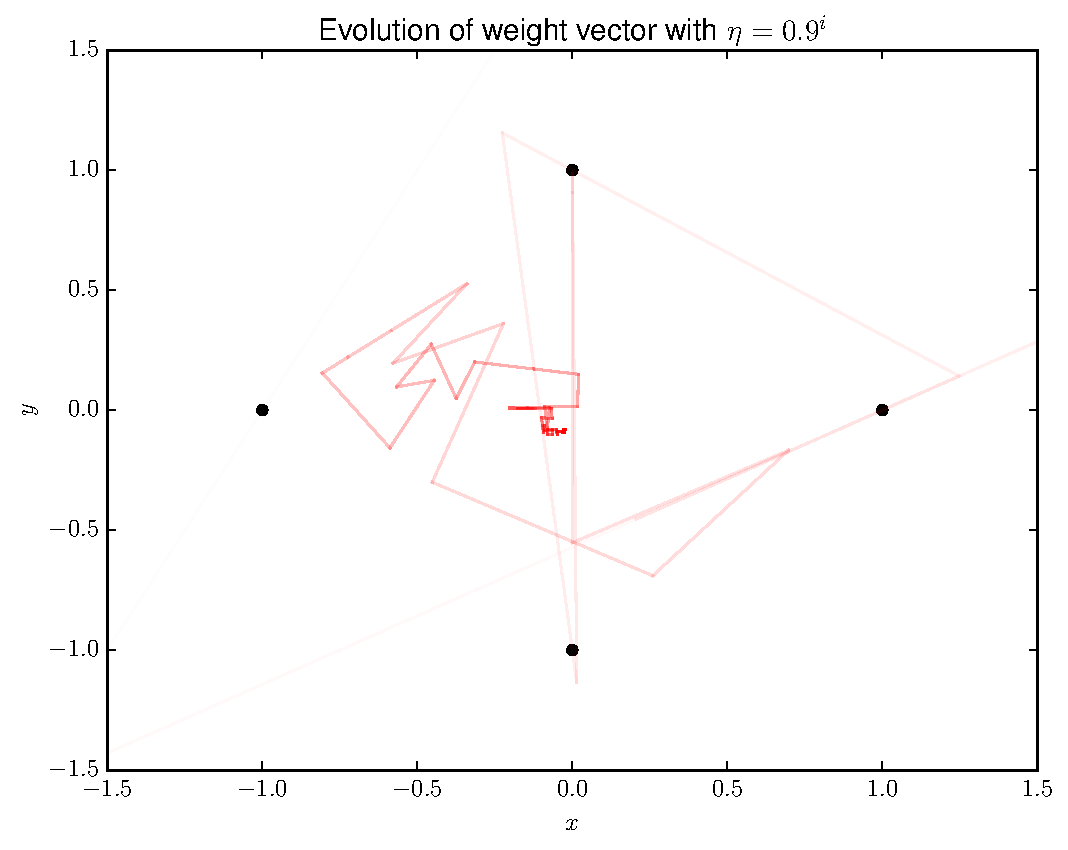
\includegraphics[width=.75\linewidth]{Decreasing.pdf}
\caption{Decreasing value of $\eta$}
\label{fig:dec}
\end{figure}


\begin{figure}[H]
\centering
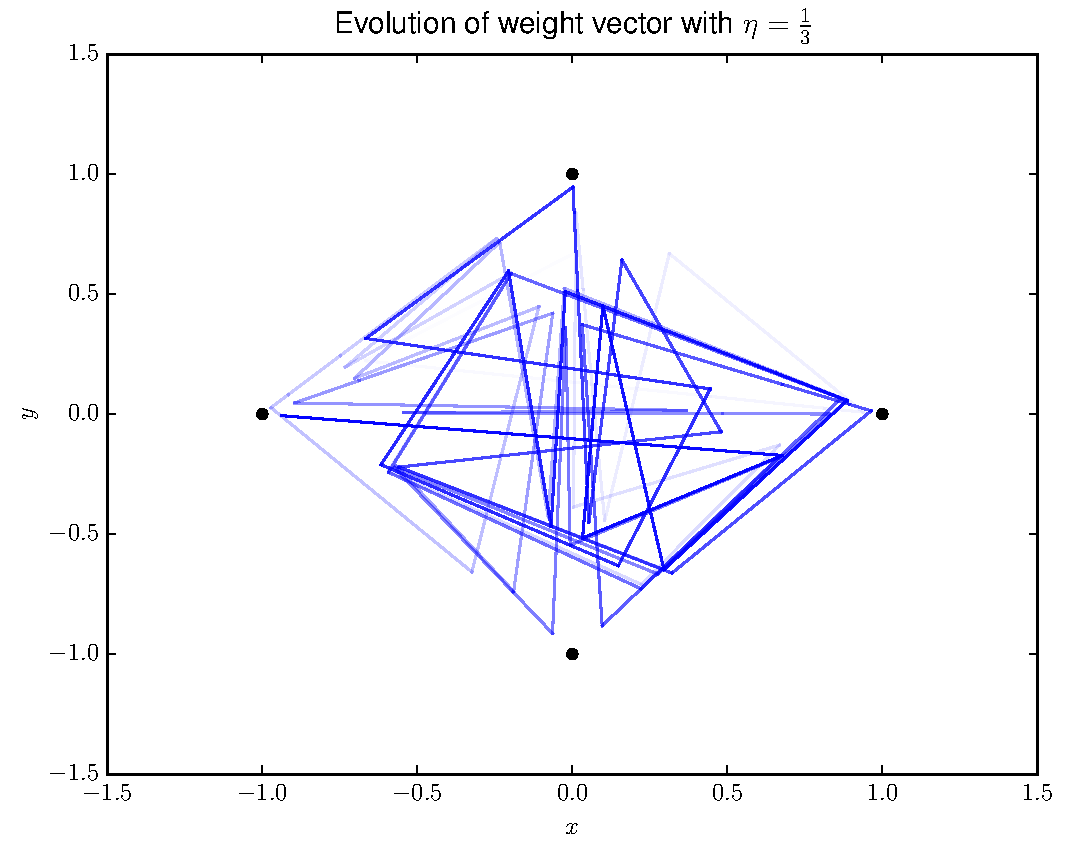
\includegraphics[width=.75\linewidth]{Fixed.pdf}
\caption{Fixed value of $\eta$}
\label{fig:fix}
\end{figure}

In the above figures, the black dots represent the data points. For the lines, the alpha channel is proportional to the iteration such that the earlier the iteration the more faint, and as the iterations progressed the alpha channel was increased. The above figures are for 20 points each for the given domain. They also used the exact same shuffled list.

As Figure~\ref{fig:dec} shows, even though $\eta$ started off with a value of $0.9$, with each iteration it was updated to be $\eta^{i}$ for the $i^{th}$ data point. In this instance, it converged rather quickly. However, with the fixed case in Figure~\ref{fig:fix}, it is easily seen that it keeps diverging from one point to the next. This is due to the {\em randomness} of SGD with the points being shuffled, and choosing the points randomly from the dataset. 

\item Pick $n = 100$ random points in $[-1, 1]^{2}$ (uniformly), and run SGD for fixed $\eta = 1/2$, as above. Write down what the distance to optimum is, after $T = \{ 10, 100, 1000\}$ iterations (if you want to be careful, you should average over $5$ random choices for the initialization). Now consider dropping the step size $\eta_{t} = 1/t$, and write down the result for $T$ as above.

      {\bf Solution:}

The algorithm implemented for SGD can be seen below

\begin{minipage}{\linewidth}
\begin{algorithm}[H]
\caption{Stoichastic Gradient Descent}\label{SGD}
\begin{algorithmic}[1]
\Input $m$ values of $\bm{x}_{i} \in \mathbb{R}^{d}$, $\bm{\theta} \in \mathbb{R}^{d}$, $T$
\Output $\bm{\theta}$ minimized over the data
\State Randomly shuffle dataset
\State Initialize values of $\bm{\theta}$
    \For{$i = 1, 2, \ldots, T$}{
      \State $\theta_{j}\gets \theta_{j} - \eta \grad_{\theta} J\P{\bm{\theta}, \bm{x}_{i}}$
      \Comment for every $j = \left\{ 0, 1, \ldots, \mathbb{R}^{d}\right\}$
    \EndFor}\\
\Return $\bm{\theta}$
\end{algorithmic}
\end{algorithm}
\end{minipage}

The following tables have the results of how far away from the minima the resulting weight vector was. It is an average taken over $5$ different examples for each value of $T$, where the data was shuffled before each iteration. 

\begin{table}[H]
\centering
\caption{Distance from the minima with $\eta = 1/2$}
\begin{tabular}{c c c}
\hline\hline
$T = 10$ & $T = 100$ & $T = 1,000$\\
\hline
0.944 & 0.592 & 0.769\\
\hline
\end{tabular}
\label{table:fix}
\end{table}

\begin{table}[H]
\centering
\caption{Distance from minima with $\eta = 1/i$}
\begin{tabular}{c c c}
\hline\hline
$T = 10$ & $T = 100$ & $T = 1,000$\\
\hline
0.218 & 0.076 & 0.063\\
\hline
\end{tabular}
\label{table:decay}
\end{table}


As the above shows, and as is to be expected, the trials with the fixed value of $\eta$ were all over the place and a larger value of $T$ did not guarentee convergence. However, with a decaying value of $\eta$, as seen in Table~\ref{table:decay}, the values did come a lot closer to the minima, and did moreso with increased values of $T$.





\end{enumerate}

\item (Numeric accuracy in MW updates) Consider the randomized experts setting we saw in class (we maintain a distribution over experts at each time, and the loss of the algorithm at that time is the expected loss over the distribution). Consider the simple setting where the experts predict $0/1$, and the loss is either $0$ or $1$ for each expert. We saw how to update the probabilities (multiply by $e^{-\eta}$ if an expert makes a mistake, keep unchanged otherwise, and renormalize). One of the common problems here is that numeric errors in such computations tend to compound if not done carefully.

Suppose we have $N$ experts, and we start with a uniform distribution over all of them. Let $p_{t}^{(i)}$ denote the probability of expert $i$ at time $t$, for the ``True'' (infinite precision) multiplicative weight algorithm, and let $q_{t}^{(i)}$ denote the probabilities that the ``real life'' algorithm uses (due to precision limitations).

\begin{enumerate}
  \item Consider one simple suggestion: Say we zero out weights that are ``too small,'' specifically, suppose we set $q_{t}^{(i)} = 0$ if $q_{t}^{(i)}/\max_{j}q_{t}^{(j)} < \epsilon$, for some precision parameter $\epsilon$ (such changes frequently occure due to roundoff). Other than this, suppose that the $q_{t}^{(i)}$ are updated accurately. Prove that in this case, we cannot hope to achieve any non-trivial regret bound. Specifically, for large enough $T$, the algorithm can have error $T(1 - \BigO{1})$, while the best expert may have error $\BigO{T}$.

[{\em Hint:} In this case, we are ``losing'' all information about an expert]

      {\bf Solution:}

\item A simple way to avoid this (in this setting) is to avoid storing probabilities, but instead maintaining only the number of mistakes $m_{t}^{(i)}$. Prove how this suffices to recover the probabilities $p_{t}^{(i)}$ (assuming infinite precision arithmetic).

      {\bf Solution:}

\item Suppse we use the idea in part $(b)$ to construct a distribution $q_{t}$ that differs from $p_{t}$ by $< \epsilon$ in the $\ell_{1}$ norm, {\em i.e.}, $\sum_{i}\abs{p_{t}^{(i)} - q_{t}^{(i)}} < \epsilon$. Then, assuming we construct such a $q_{t}$ at time $t$ to sample, show that the expected number of mistakes of the algorithm is bounded by $(1 + \eta)\min_{i}m_{T}^{(i)} + \BigO{\log(N)/\eta} + \epsilon T$.

      {\bf Solution:}

\item The bound above is not great if there is an expert who makes very small number of mistakes (compared to $T$). Noting that we are dealing with binary predictions, can you come up with a way to run the algorithm, so as to obtain a mistake bound of $\left( 1 + \eta + 2\epsilon\right)\min_{i}m_{T}^{(i)} + \BigO{\log(N)/\eta}$?

      {\bf Solution:}

\end{enumerate}
\end{enumerate}
 
\end{document}